%\vspace{-0.05in}
\section{Understanding Application Memory Use}
\label{constrainedcapacity}
%\vspace{-0.05in}

\begin{figure}[t]
    \centering
    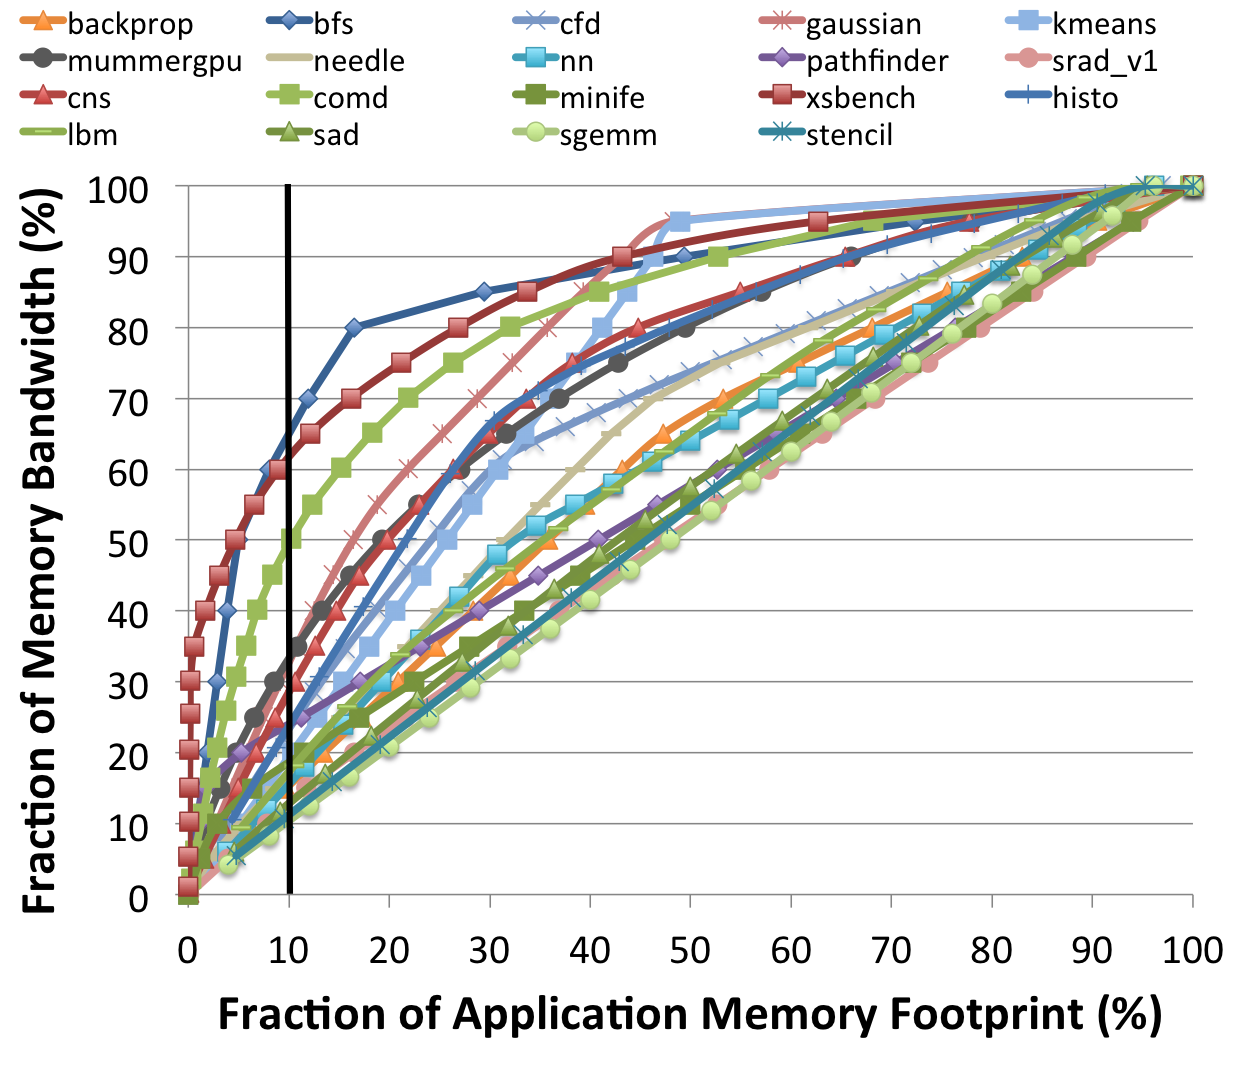
\includegraphics[width=0.9\columnwidth]{asplos2015/figures/cdf.png} 
    \caption{Data bandwidth cumulative distribution function with pages sorted from hot (most memory accesses) to cold (least memory accesses).}
    \label{fig:cdf}
\end{figure}

Section~\ref{bwawareplacement} showed that optimal BW-AWARE placement requires
the majority of the application footprint to fit in the bandwidth-optimized memory
to match the bandwidth service ratios of the memory pools.
However, as shown in Figure~\ref{fig:arch}, systems may have bandwidth-optimized
memories that comprise less than 10\% the total memory capacity, particularly those using
on-package memories which are constrained by physical dimensions. If the application footprint
grows beyond the bandwidth-optimized capacity needed for BW-AWARE placement, the operating system
has no choice but to steer remaining page allocations into the capacity-optimized memory.
Unfortunately, additional pages placed in the CO memory will skew the
ratio of data transferred from each memory pool away from the optimal BW-AWARE ratio.

For example, in our simulated system if the bandwidth-optimized memory
can hold just 10\% of the total application memory footprint, then a BW-AWARE placement would end up placing
10\% pages in the BO memory; the
remaining 90\% pages must be spilled exclusively to the capacity-optimized memory.  This ratio of
$90C$-$10B$ is nearly the inverse of the performance-optimized ratio of $30C$-$70B$.  
To improve upon this capacity-induced placement problem, we recognize
that not all pages have uniform access frequency, and we can selectively place
hot pages in the BO memory and cold pages in the CO memory. 
{\color{black}In this work we define page \textit{hotness} as the number of accesses to that page that 
are served from DRAM.}


\subsection{Visualizing Page Access Distribution}
\label{annotation}
%\vspace{-0.05in}
Figure~\ref{fig:cdf} shows the cumulative distribution function (CDF) 
for memory bandwidth as a fraction of the total
memory footprint for each of our workloads. The CDF was generated by counting
accesses to each 4kB page, after being filtered by on-chip caches, and then sorting
the pages from greatest to least number of accesses.
Applications that have the same number of accesses to all
pages have a linear CDF, whereas applications in which some pages are accessed
more than others have a non-linear CDF skewed towards the left of the
graph. For example, we see that for applications like {\tt bfs} and {\tt xsbench}, over 60\% of
the memory bandwidth stems from within only 10\% of the application's allocated pages.  Skewing the 
placement of these hot pages towards bandwidth-optimized memory will improve the performance
of GPU workloads which are capacity constrained by increasing the traffic to the bandwidth-optimized 
memory. However, for applications which have linear CDFs, there is little headroom for 
improved page placement over BW-AWARE placement.

\begin{figure}[t]
    \centering
    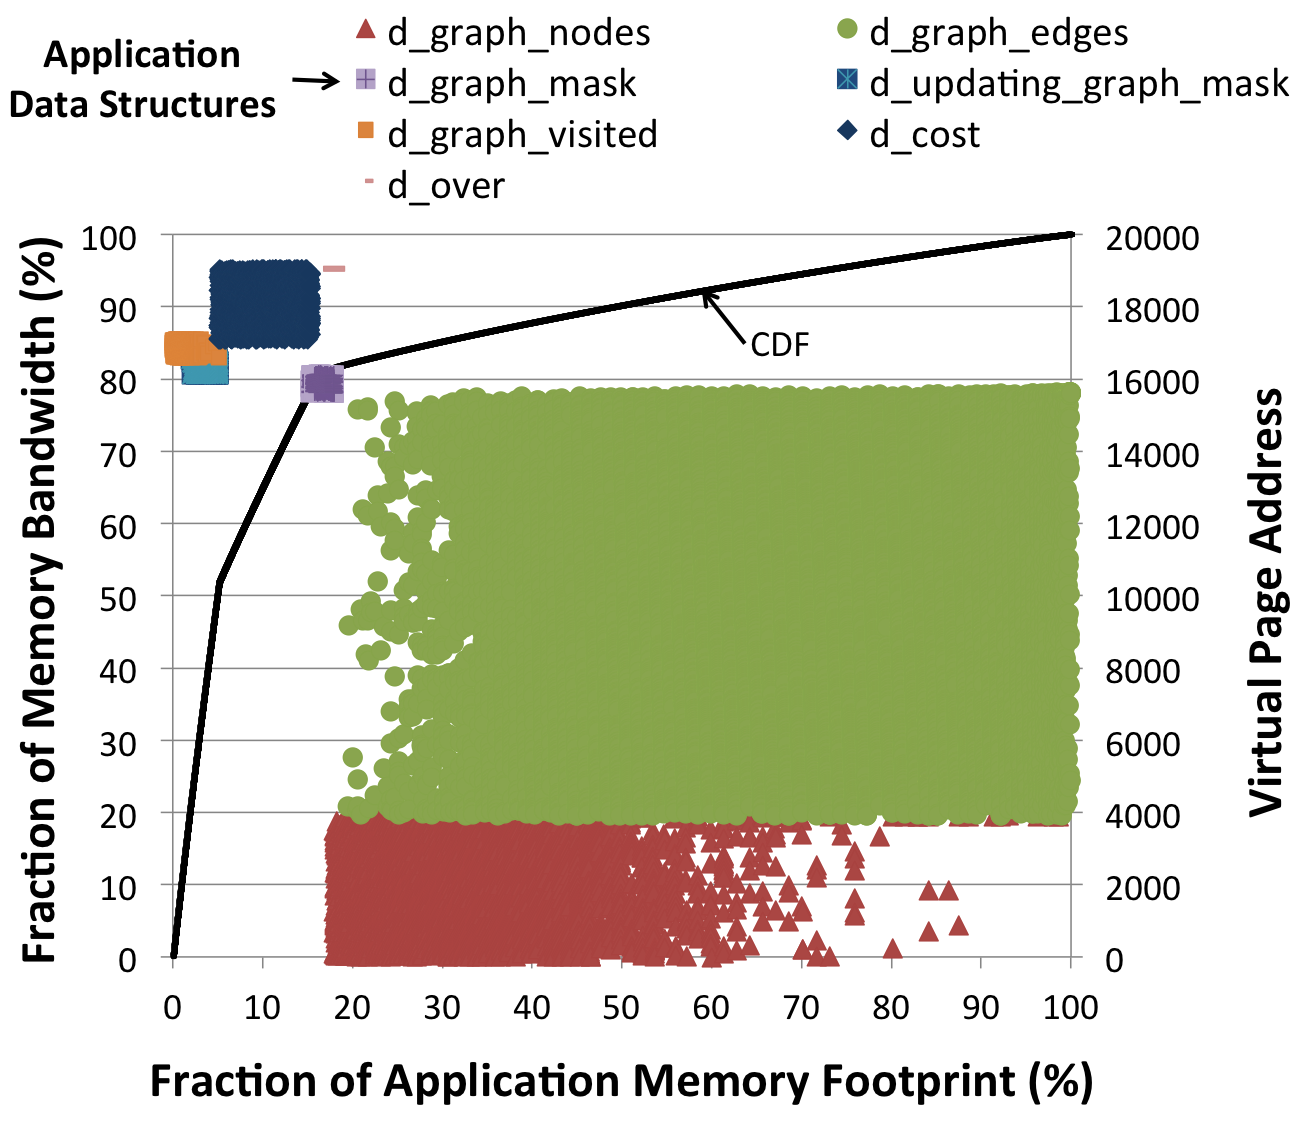
\includegraphics[width=0.9\columnwidth]{asplos2015/figures/bfsannotated.png}
    \caption{{\tt bfs}: CDF of data footprint versus virtual address data layout.}
    \label{fig:cdfannotation-bfs}
\end{figure}

Figure~\ref{fig:cdf} also shows that some workloads have sharp inflection points
within the CDF, indicating that distinct ranges of physical addresses appear to
be clustered as hot or cold. To determine if these inflection points could be
correlated to specific memory allocations within the application, we plotted the
virtual addresses that correspond to application pages in the CDF, and then
reverse-mapped those address ranges to memory allocations for program-level data
structures, with the results shown in
Figure~\ref{fig:cdfannotation-bfs},~\ref{fig:cdfannotation-muumergpu},~\ref{fig:cdfannotation-needle}\@.
{\color{black} The x-axis shows the fraction of pages allocated by the
application, where pages are sorted from greatest to least number of accesses.
The primary y-axis (shown figure left) represents the CDF of memory bandwidth
among the pages allocated by the application (also shown in
Figure~\ref{fig:cdf}).  Each point on the secondary scatter plot (shown figure
right) shows the virtual address of the corresponding page on the x-axis. The
points (pages) are colored according to different data structures they were
allocated from in the program source.}

\begin{figure}[t]
    \centering
    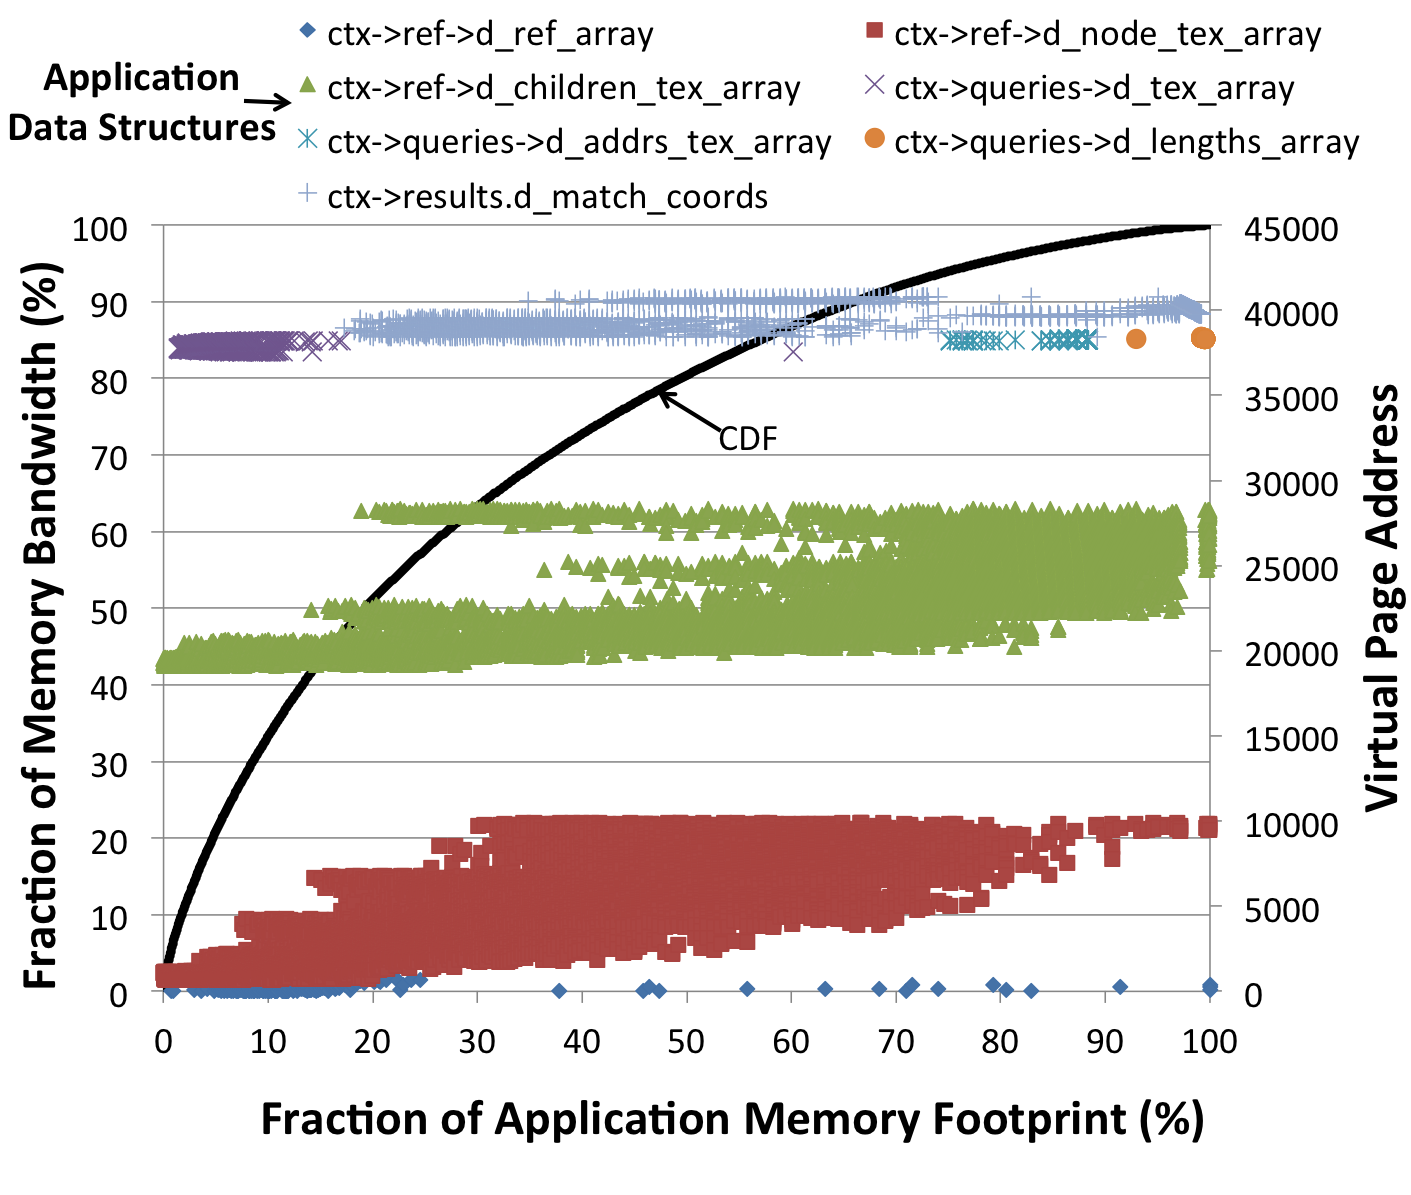
\includegraphics[width=0.9\columnwidth]{asplos2015/figures/mummerannotated.png}
    \caption{{\tt mummergpu}: CDF of data footprint versus virtual address data layout.}
    \label{fig:cdfannotation-muumergpu}
\end{figure}

We analyze three example applications, {\tt bfs, mummergpu}, and
{\tt needle} which show different memory access patterns. For {\tt bfs}, we can
see three data structures: {\tt d\_graph\_visited}, {\tt
d\_updating\_graph\_mask}, and {\tt d\_cost} consume {\color{black}$\approx80\%$
of the total application bandwidth while accounting for $\approx20\%$} of the
memory footprint.  However for {\tt mummergpu}, the memory hotness does not seem
to be strongly correlated to any specific application data structures. Several
sub-structures have similar degrees of hotness and some virtual address ranges
(10,000-19,000 and 29,000-37,000) are allocated but never never accessed. In
{\tt needle}, which has a fairly linear CDF, the degree of memory hotness
actually varies within the same data structure. While we examined all
applications with this analysis, we summarize our two key observations.

\begin{figure}[t]
    \centering
    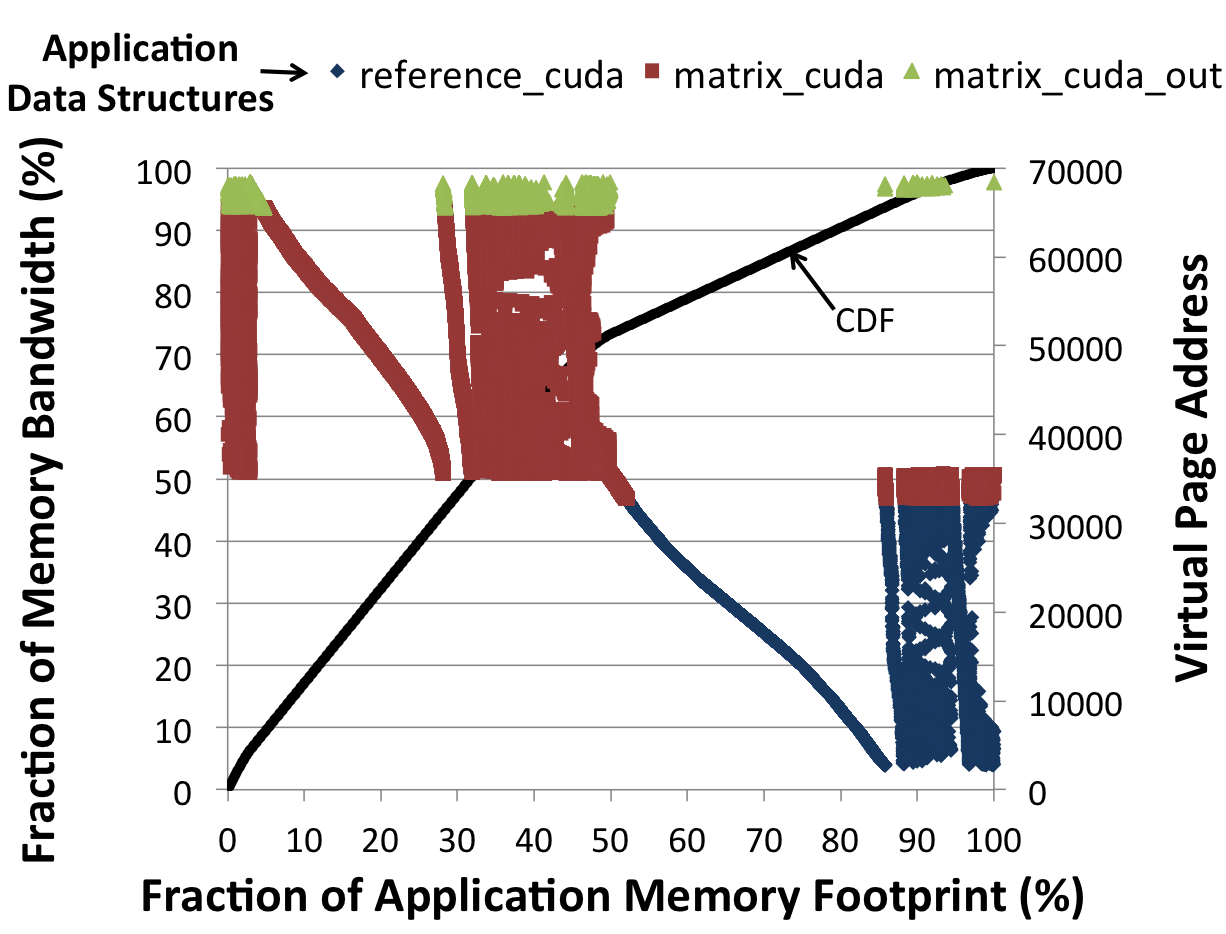
\includegraphics[width=0.9\columnwidth]{asplos2015/figures/needleannotated.png}
    \caption{{\tt needle}: CDF of data footprint versus virtual address data layout.}
    \label{fig:cdfannotation-needle}
\end{figure}

\emph{Individual pages can and often do have different degrees of hotness}.
Application agnostic page placement policies, including BW-AWARE placement, may leave performance 
on the table compared to a placement policy that is aware of page frequency distribution. 
Understanding the relative hotness of pages
is critical to further optimizing page placement.  If an application does not have a skewed CDF, 
then additional effort to characterize and exploit hotness differential will only introduce 
overhead without any possible benefit.

\emph{Workloads with skewed cumulative distribution functions often have sharp
distinctions in page access frequency that map well to different application 
data structures.}  Rather than attempting to detect and segregate individual physical pages 
which may be hot or cold, application structure and memory allocation policy
will likely provide good information about pages which will have similar degrees of hotness.

\subsection{Oracle Page Placement}
With knowledge that page accesses are highly differentiated for some applications, we implemented
an oracle page placement policy to determine how much more application performance could be achieved
compared to BW-AWARE placement in capacity constrained situations.  {\color{black}Using perfect knowledge of page
access frequency, an oracle page placement policy will allocate the hottest pages possible into the
bandwidth-optimized memory until the target bandwidth ratio is satisfied, or the capacity of this memory
is exhausted.}  We implemented this policy using two phase simulation. First, we obtained perfect
knowledge of page access frequency. Then in a second simulation pass, we used this information to allocate
pages to achieve the best possible data transfer ratio under a 10\% capacity constraint where only
10\% of the application memory footprint fits within the bandwidth-optimized memory.

\begin{figure}[t]
    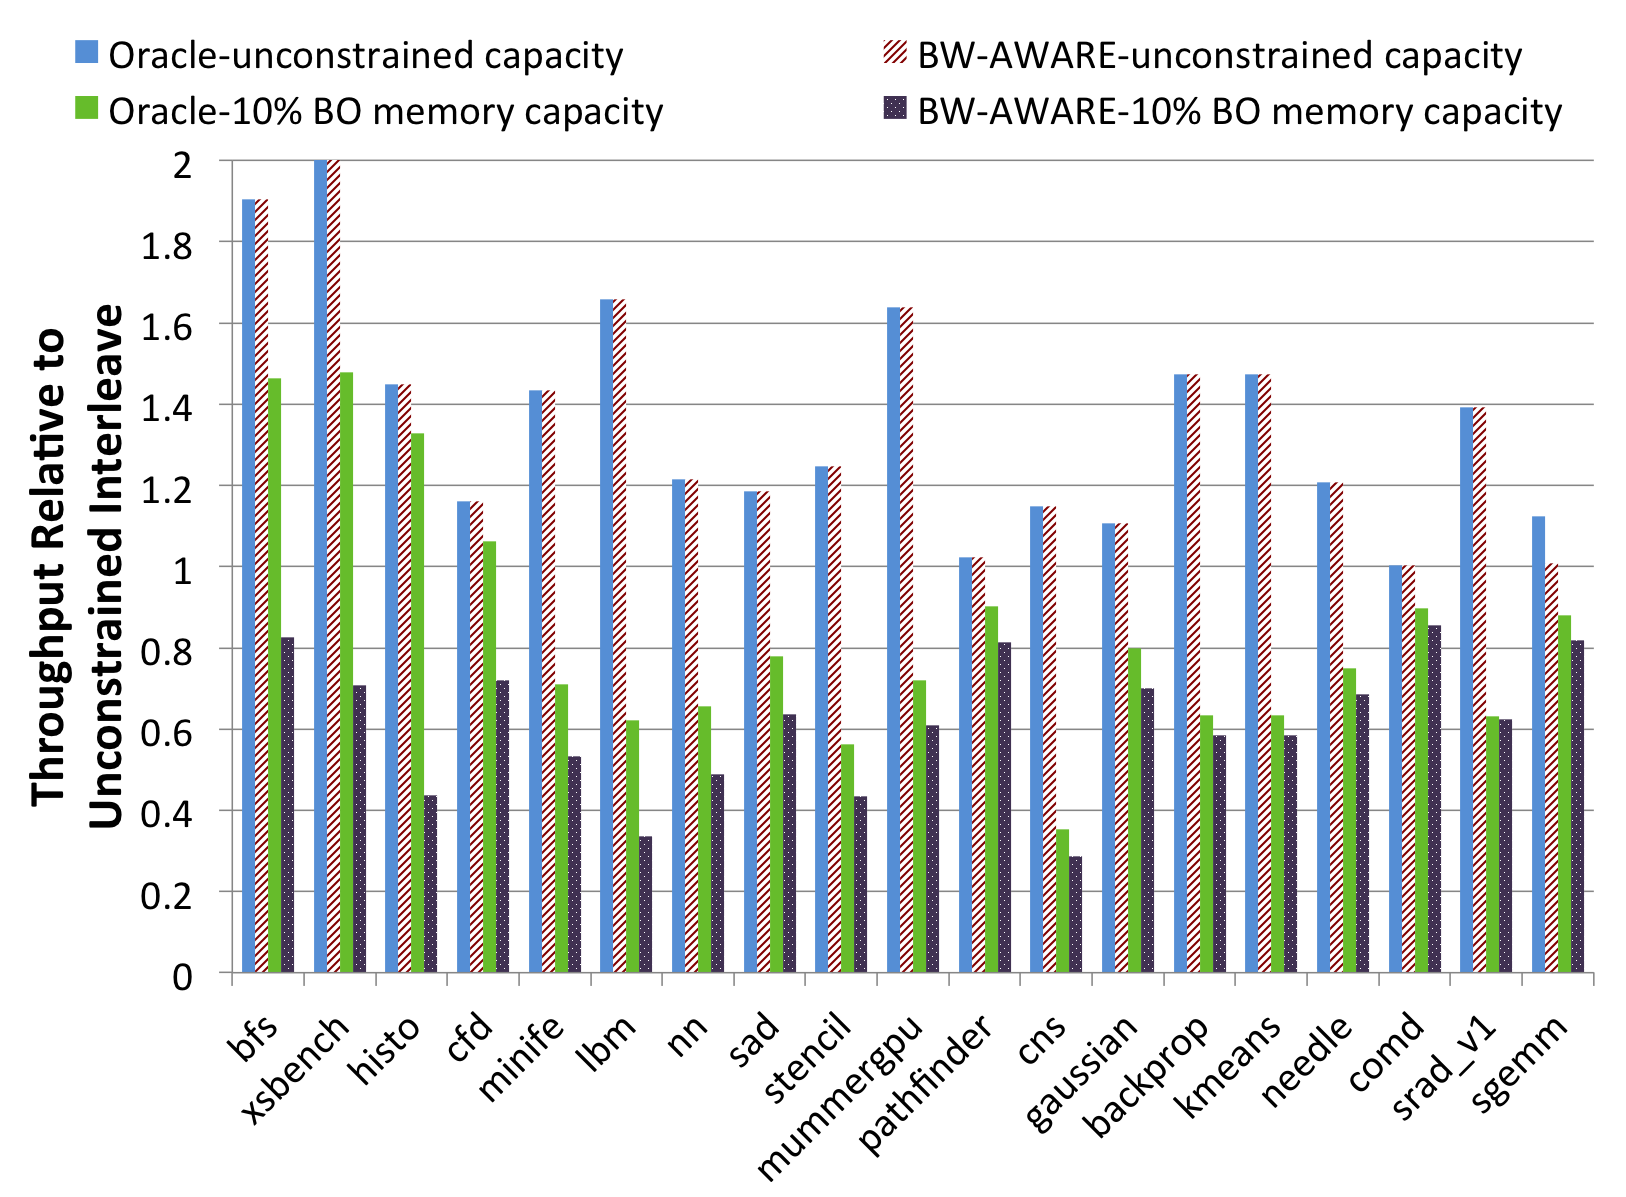
\includegraphics[width=\columnwidth]{asplos2015/figures/oracle-perf.png} 
    \caption{Oracle application performance of a constrained capacity system vs
unconstrained capacity system}
    \label{fig:oracleperf}
\end{figure}

{\color{black}Figure~\ref{fig:oracleperf} compares the performance of the oracle and BW-AWARE
placement policies in both the unconstrained and 10\% capacity constrained
configuration.  Figure~\ref{fig:oracleperf} confirms that BW-AWARE placement is
near-optimal when applications are not capacity limited.  This is because both BW-AWARE
and oracle placement are both able to achieve the ideal bandwidth distribution, though
the oracle policy is able to do this with a smaller memory footprint by placing fewer, hotter, pages in the BO memory.
Under capacity constraints, however, the oracle policy can nearly double the performance of the BW-AWARE policy for applications
with highly skewed CDFs and it outperforms BW-AWARE placement in all cases. This because the random
page selection of BW-AWARE placement is not able to capture enough hot pages for placement in BO
memory, before running out of BO memory capacity, to achieve the ideal bandwidth distribution.  
On average the oracle policy is
able to achieve nearly 60\% the application throughput of a system for which there is no capacity
constraint.  This additional performance, achievable through application awareness of memory
access properties, motivates the need for further improvements in memory placement policy.}
